\documentclass[12pt, a4paper]{article}
\pagenumbering{arabic}
\usepackage[utf8]{inputenc}
\usepackage[T1]{fontenc}
\usepackage{geometry}
\usepackage{graphicx}
\graphicspath{{images/}}
\geometry{a4paper}
\usepackage{helvet}
\newcommand\tab[1][1cm]{\hspace*{#1}}
\renewcommand{\familydefault}{\sfdefault}
\setlength{\topmargin}{-2cm}
\setlength{\oddsidemargin}{0cm}
\setlength{\textheight}{24cm}
\setlength{\textwidth}{16cm}
\usepackage{graphicx}
\usepackage{listings}
\usepackage{sectsty}
%Use Helvetica as the sansserif font
\usepackage{helvet}
%Use sffamily for all titles
\allsectionsfont{\sffamily}
\begin{document}
\title{WiFi SPOTS IN MAKERERE UNIVERSITY KAMPALA (MUK)}
\author{WANYAMA SIMON PETER }
\maketitle
\clearpage
\section{Abstract}
The aim of this study was to acquire information about the most frequently used WiFi spots around the compound of Makerere University Kampala. A survey about locations, signal strength, and user experience, and user ratings was carried out. The results indicate that the major problem is with the convinience of the place where to sit while surfing and low speeds during day time since many people are active. The report concludes with a tally of the results showing some spots more reliable than others. It also recommends improvement with additional access points and also constrction of shades and better rlelaxing gardens for convinience while students and other users surf. 

\section{Introduction}
There has been massive increase in demand for internet by students since it provides vast sources of information required in the daily reseaech to answer assignments and courseworks and also to interconnect from different places of the world. It also provides entertainment which releaves students' stress, It's is akso a great aid of to communication for example social media.\\
 \\
Most times, some students mostly those who commute from far places find it hard to find the WiFi spots where they can get convinience and and reliability to do their surfing. Some of these face the problem of failing courseworks due to little research, fighting for the fewer books as compared to the number of students in the library, they tend to gain little knowledge, they also fail to submit their online assignments on time and face the penalty.\\
\\
 For the purposes of this research study, WiFi spot means a place near the wifi access point where one can go and find signal and connect to the wireless network and surf

\section{Methodology}
This reseach study was conducted using an Android phone Mobile Application called ODK collect through four major ways; Interviewing, Taking GPS Coordinates, Physical testing through using by the reseacher himself, taking pictures. Data including Where the WiFi spot is located, the GPS coordinates, Average Number of Users, Pictures, Security passwords, Average Speed, Average rating by users, other user views in audio and convinience of the place where people can surf from have been used to analyse the Wifi spots around MUK.
\newline The WiFi spots analyzed included Halls of residence of Mitchell, Nkrumah, University Hall, Lumumba, and Livingstone. Places like School of Computing, Gender, Library were also part of the study.
\subsection{ScreenShots of Mobile Phone Application}

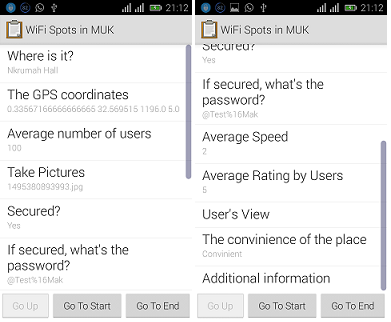
\includegraphics{shot3}

\section{Results}
There was 70 percent response by the users who were interviewed and these conntributted to the Audio files and ratings by users, All other data was also just collected with Ease. From the table below, it can be seen that there are some better places that students should maximize and avoid over crowding places with weaker network. 
\subsection{Tabular Summary of Results}
\begin{center}
\begin{tabular}{|| c | c | c | c | c ||}
\hline \textbf{Wifi Spot} & \textbf{No. of Users} & \textbf{Average speed$_{mbps}$} & \textbf{Rating /10} & \textbf{Convinience}\\
[0.5ex]
\hline
\hline Mitchell & 130 & 5 & 6 & Good\\
\hline UH & 100 & 6 & 7 & Very Good\\
\hline Livingstone & 90 & 7 & 7 & Very Good\\
\hline Gender & 80 & 7 & 6 & Good\\
\hline SCIT & 100 & 4 & 4 & Good\\
\hline Lumumba & 100 & 5 & 7 & Good\\
\hline FEMA & 150 & 3 & 4 & Bad\\
\hline Nkrumah & 100 & 6 & 7 & Fair\\
\hline Pharmacy & 70 & 8 & 8 & Excellent\\
[0.5ex]
\hline 
\end{tabular}
\end{center}

\section{Conclusion}
The use of WiFi is inevitable in the modern world as its the major source of information, and to students it's more than just inevitable. i therefore urge any of them reading this piece of document to take advantage of the most convinient and faster spots of WiFi in Makerere University. 

\section{Recommendation}
Its recommended that The WiFi lovers to take up the spots with faster and convinient places for a better experience.
I also recomment for the improvement of the places where people sit to surf and improvement of the network as a whole as by increasing speed and also the university should also build bulid more access points to avoid crowding of students in some places.
\clearpage

\begin{thebibliography}{1}
\bibitem{} N. Robberts {\em  Research Methodology Concepts} 2004. RMIT
\bibitem{} http://www.wifi-spots-in-muk.appspot.com
\end{thebibliography}

\end{document}
